\section{Feedforward Neural Network Architecture} \label{sec:feedforward_nn}

Feedforward neural networks are the most basic type of deep learning model. Feedforward networks are designed to approximate a function that best maps the network's input to its output \cite{lecun2015deep}. On a high level, a feedforward neural network algorithm has four phases. The first phase is forward propagation, where the data flows through the network and initializes every node's values. The second phase is error evaluation, which determines how well the network performs with its current nodes' value. The third phase is gradient descent, where the algorithm determines which part of the network causes it to perform poorly. The last phase is backpropagation, where the algorithm updates the node's value in the network to make it more accurate and better fit the input data set. These four phases are applied and repeated on an extensive data set to become more accurate over time. We discuss each phase of the algorithm in this section, but we first need to understand the basic structure of a feedforward neural network.

\subsection{The Network Structure \label{network_structure}}
% \hl{Network layer}
To understand the feedforward network structure, we first define the idea of layers in the context of ANN. A \textbf{layer} in a neural network is a collection of neuron nodes at a specific network depth. A layer is represented by a column of nodes in Figure \ref{fig:fc_ffn}. A feedforward network can be thought of as a stack of multiple layers. Each layer in the stack is responsible for transforming the layer's input to help make sense part of the representation for later layers. At a high level, the network consists of the \textbf{input layer}, single or multiple \textbf{hidden layers}, and the \textbf{output layer}. The number of hidden and output layers is the \textbf{depth} of the network. As an example, Figure \ref{fig:fc_ffn} is a fully connected feedforward neural network with a depth of three.

\begin{figure}[!ht]
    \centering
    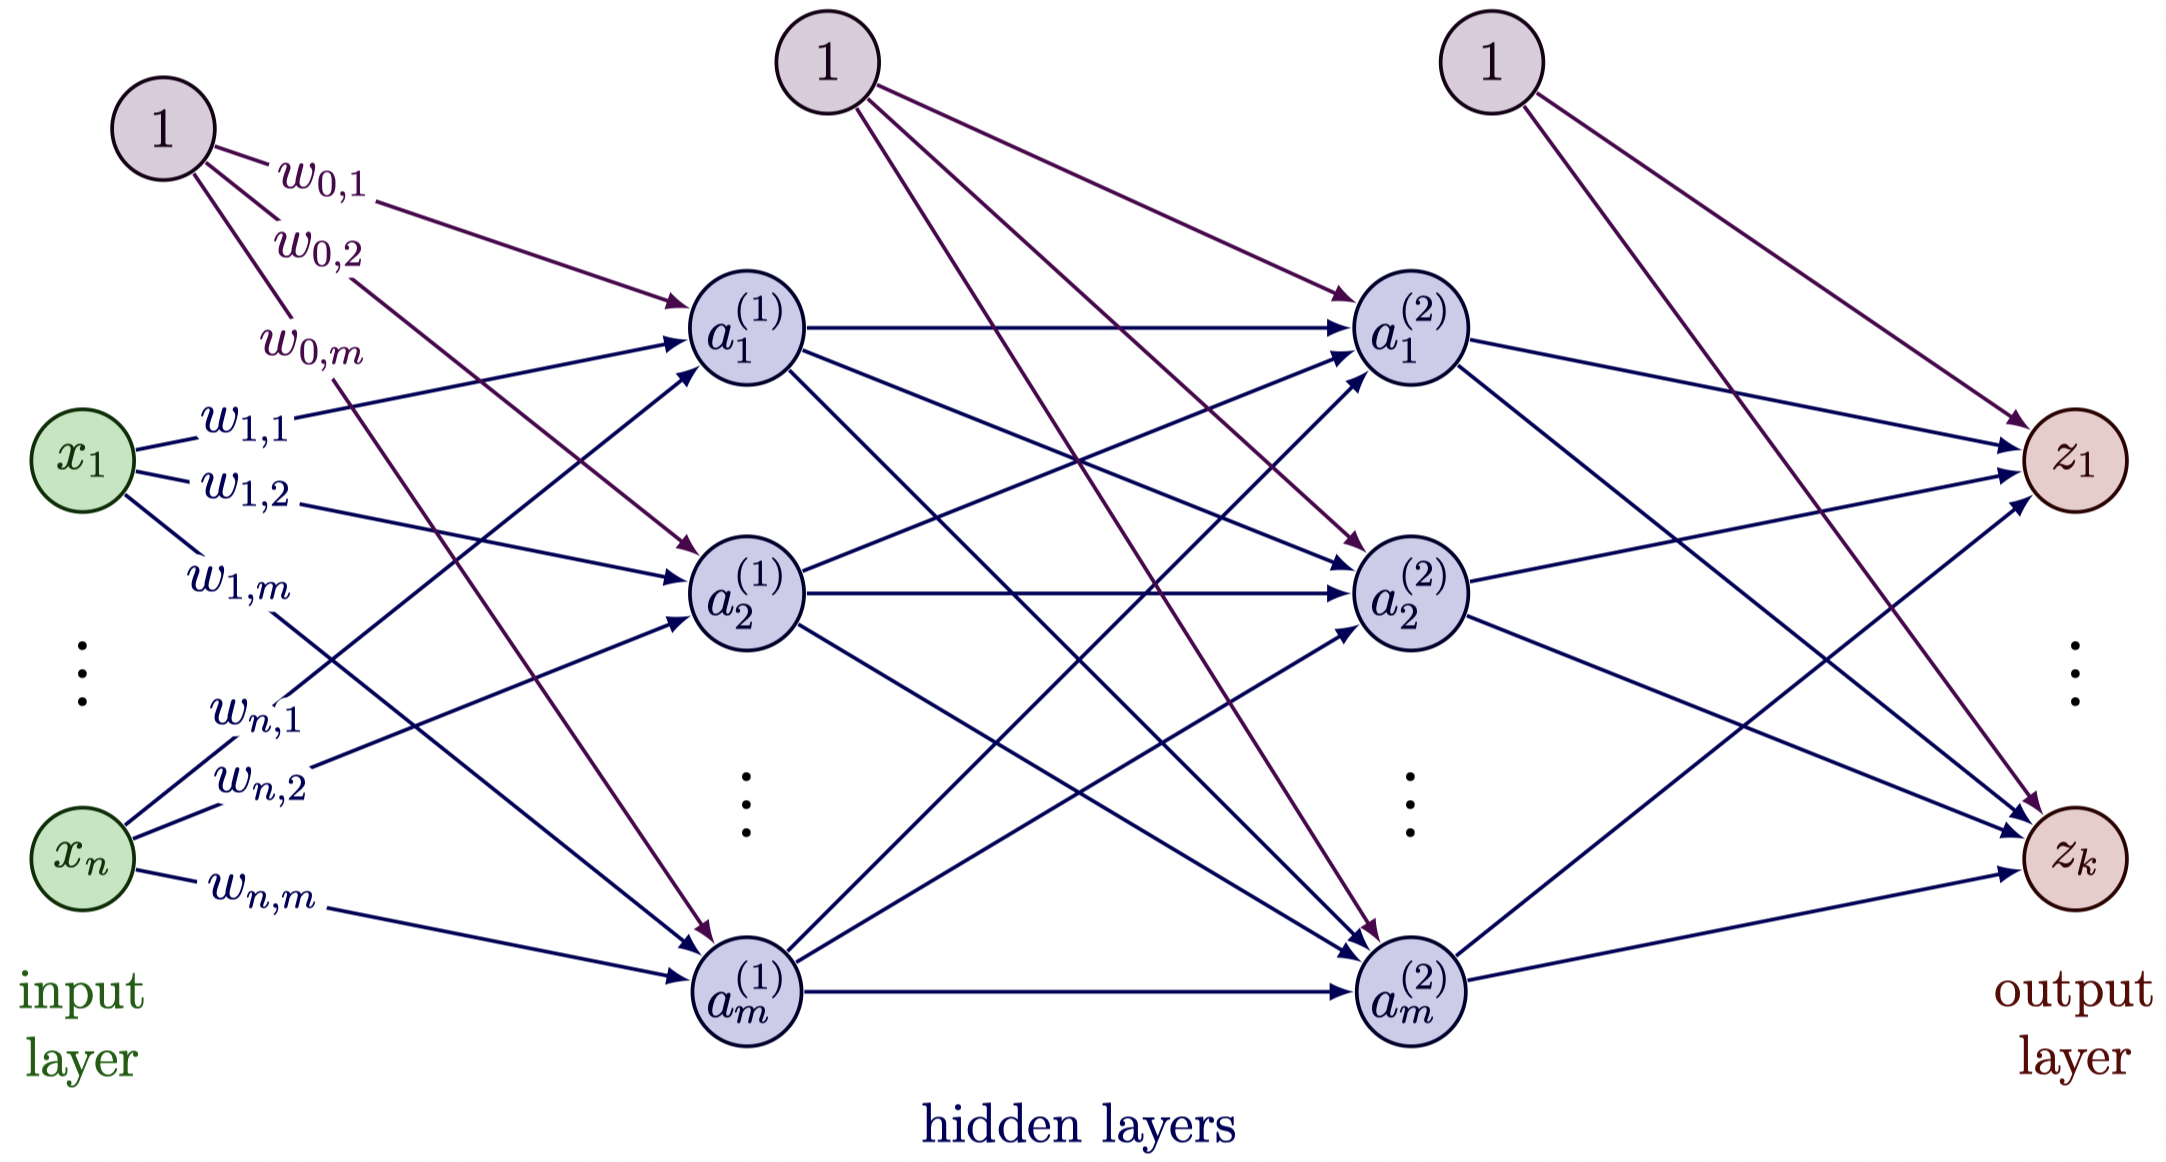
\includegraphics[width=5in]{figures/ffn_diagram.png}
    \caption{A Fully Connected Feedforward Neural Network} \label{fig:fc_ffn}
\end{figure}

% \hl{Network neuron + activation signal}
Each layer consists of one or more nodes. Each node in a layer represents an \textbf{artificial neuron}. The number of neurons in each layer can be different from one another. Each neuron holds a numerical value called the \textbf{activation signal}. In theory, the activation signal takes on any value in the real numbers set $\mathbb{R}$. However, in practice, studies have shown multiple advantages when normalizing the activation signal of every neuron \cite{lecun2012efficient}. As an example, we consider a network that receives a $23 \times 23$ RGB image and then produces a dog or cat label for the object in the image. In the input layer, the number of neurons is the total pixel in the image in each color channel, that is $23 \times 23 \times 3$ neurons, and each neuron (denoted $x_i$) holds that pixel value normalized. On the other hand, the output layer only has two neurons (denoted $z_i$); one corresponds with the dog and the other with the cat. Unlike the input and output layers, where the number of neurons needed is straightforward, the number of neurons in each hidden layer and the number of hidden layers are complicated to determine and remain outside the scope of this paper. However, studies have shown that networks with the same number of neurons in hidden layers perform better \cite{taylor2017neural}, and deeper networks result in more advanced learning with some issues like gradient vanishing \cite{lecun2015deep}.

% \hl{Network connection + weight}
Each neuron in a layer affects a neuron from the next layer through a \textbf{connection}. The connection is represented by a line between two neurons in Figure \ref{fig:fc_ffn}. In fully connected networks, each neuron in a layer is affected by all the neurons in the previous layer. In other words, each neuron has a connection with every neuron in the previous and the next layer of the network. Associated with each connection is a numerical value representing the \textbf{weight}. The weight of a neuron affects the influence the neuron has on the next layer of the neural network. A small weight value means the activation signal of this neuron has a low effect on neurons in the next layer. On the other hand, a high weight value results in a more significant effect proposed by this neuron to the next layer and the network's output. When a neural network algorithm initializes, its weights are randomly assigned using a Gaussian or uniform distribution \cite{lecun2015deep}. These weights are adjusted as the neural network algorithm processes to best approximate its mapping function. The weight from neuron $a_i$ to a neuron $a_j$ in the next layer is denoted as $w_{i,j}$ with the exception of bias's weight.

% \hl{Network bias}
In addition to the weight, neurons in each layer other than the input layer are also influenced by a \textbf{bias node}. A bias node is represented by a node that always holds the value 1. The bias node has connections to every neuron in the layer it affects. Each bias's connection also has a weight associated with it. The connection between bias and neuron $a_j$ in the affected layer has its weight denoted as $w_{0,j}$. The role of the bias node is like a threshold to the neuron. In other words, the bias determines how large the activation signal must be before that neuron gets propagated to the next layer of the network \cite{taylor2017neural}. Similar to weight, when the network initializes, the bias's weight is randomly assigned a value, and this value is optimized as the algorithm process. In the forward process of the network, the algorithm will compute a net input that requires a multiplication between a neuron activation signal and its weight. Since the bias node always has an activation signal of 1, thus the bias weight is the variable that directly affects nodes in the next layer. Therefore, the bias's weight is often referred to as bias.

These basic building blocks create the internal structure of a feedforward neural network. Some internal parts are also known as \textbf{internal variables or network parameters}. The model parameters refer to variables that are learned during the gradient descent process, and they are not set manually by the developers. Weights and bias weights are examples of the network's parameters. In contrast with parameters, hyperparameter refers to variables manually set by the developers and sometimes can be optimized through training \cite{lecun2015deep}. Examples of hyperparameters are the learning rate and batch size, which we will touch on more in the gradient descent section.

% \hl{Hook to forward propagation}
With the basic structure of the fully connected feedforward neural network in mind, we will discuss the first phase of an ANN algorithm. That phase is forward propagation.

\subsection{Forward Propagation} \label{forwardprop_section}
Forward propagation refers to the process by which the data move from the input layer to the output layer of the network. Regarding the image classification problem, the forward propagation process moves a list of raw pixel values through the network and gives out a number for each class label. These numbers are the \textbf{network's raw ouput}, and each number represents how likely the image is a member of this class. The forward propagation process uses two functions to evaluate the activation signal of each neuron in hidden and output layers. These two functions are the \textbf{summation function} and the \textbf{activation function} \cite{taylor2017neural}.

\begin{wrapfigure}{l}{2.5in}
    \centering
    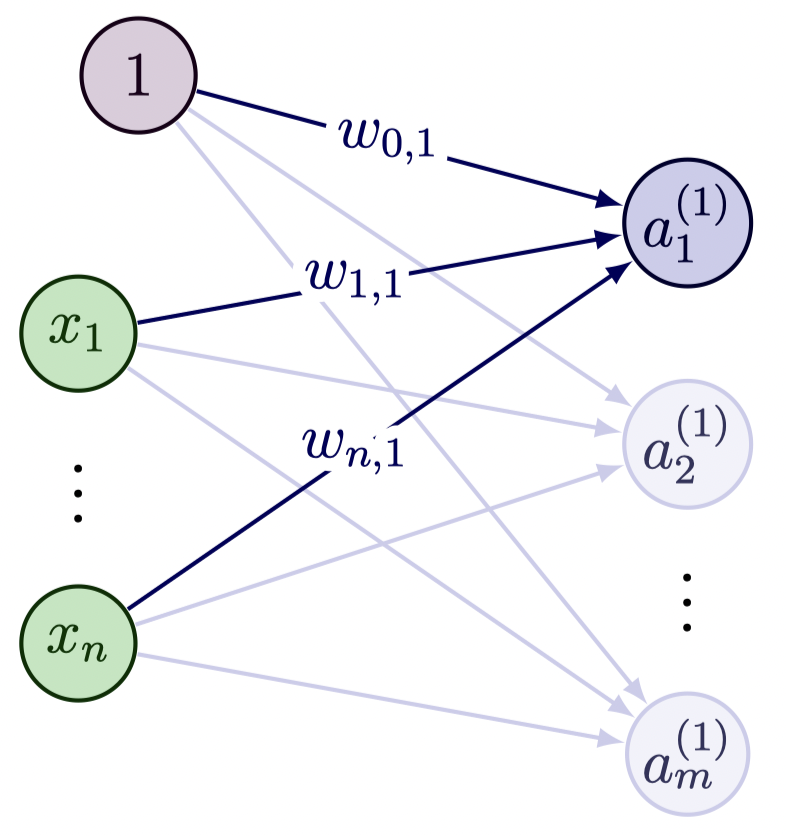
\includegraphics[width=2in]{figures/fp_diagram.png}
\end{wrapfigure}

% \hl{Summation function}
\noindent In a fully connected network, the summation function combines all neurons and their weight from the previous layer to create the net input for the current neuron. In general, the summation function is expressed as \[net\ input\ of\ a_j = \sum_{i=1}^n (x_i w_{i,j}) + 1 \cdot w_{0,j}\] where $a_j$ represents the neuron that has the summation function compute its net input \cite{taylor2017neural}. The neuron's net input is then transformed by an activation function.

% \hl{Activation func}
The activation function is responsible for transforming the net input into an activation signal, indicating if this neuron will affect later network layers. Additionally, linear functions are closed under addition; that is, adding or subtracting multiple linear functions from or to another function results in a linear function. This fact implies that the feedforward network must have non-linearity terms if it approximates a non-linear function. The use of the activation function enables the network to introduce non-linearity terms to the algorithm. Furthermore, studies have shown that the output of a network - a network that only uses a linear activation function or does not use an activation function - will be a linear combination of its input, which means hidden layers have no effect \cite{He_2015_ICCV}.

% \hl{Most common activation function} 
There are numerous activation functions proposed, each with different strengths and weaknesses. However, in practice, there are four functions and their variants that are widely used by the ANN algorithm. These four activation functions are linear, sigmoid, hyperbolic tangent (tanh), and rectified linear unit (ReLU). The formula and graphical representation of each function are shown in Table \ref{acti_func_table}.

\begin{figure}[!ht]
    \centering
    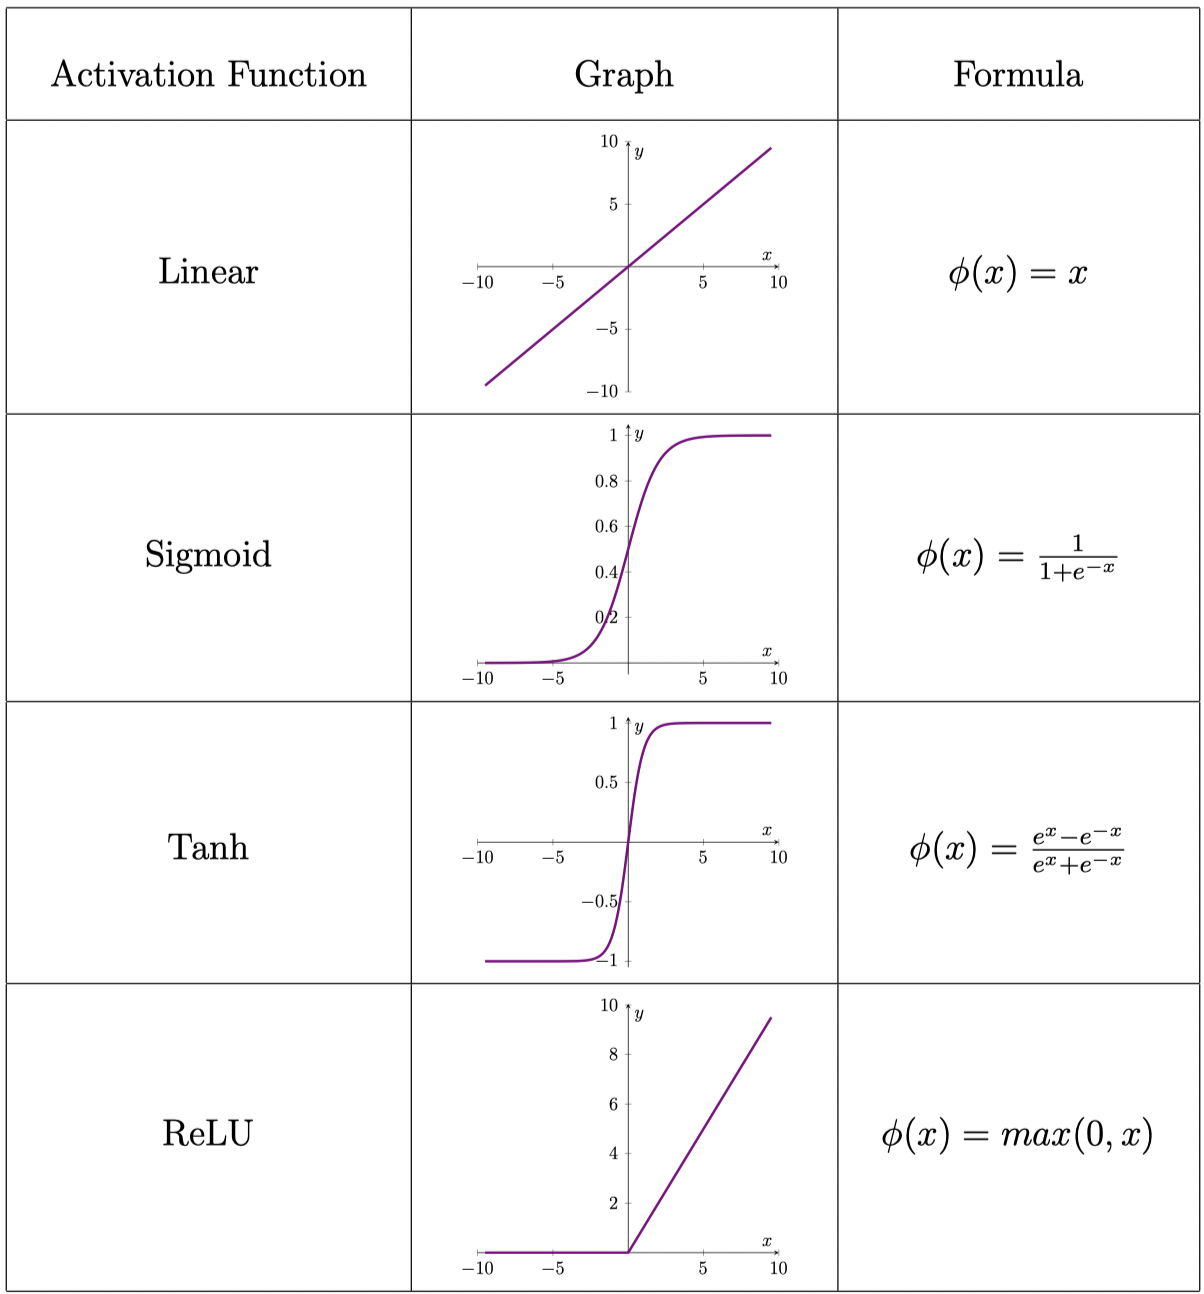
\includegraphics[width=5in]{figures/acti_func_table.png}
    \caption{Most Common Activation Function}
    \label{acti_func_table}
\end{figure}

% \hl{Activation func strength + weakness - need rewrite?} 
To understand which activation function to choose for a network, we need to know some important strengths and weaknesses of each function. First of all, the linear function is simple; thus, it is forgiving and undemanding about the resources required for training compared to other activation functions. However, the linear function is close under addition; thus, the network will only be able to approximate a linear mapping function. In contrast, sigmoid and tanh are non-linear functions, thus allowing the network to approximate a non-linear mapping function. Additionally, the sigmoid and tanh map the real number set to (0, 1) and (-1, 1), respectively. The mapping of sigmoid and tanh allow the activation signal to be normalized, thus improving training time and avoiding exploding gradients \cite{lecun2015deep}. However, the mapping also causes sigmoid and tanh to suffer from vanishing gradients problems. Different from sigmoid and tanh, ReLU maps positive signals to itself, thus able to avoid the vanishing gradients problems. The first disadvantage of ReLU is it does not have any upper bound, which requires the network to have some additional normalization layer like batch normalization (BN), weight normalization (WN), and layer normalization (LN) to optimize the training process \cite{relu_optimization_2020}. The second disadvantage of ReLU is it suffers from the dying ReLU problem, which is caused by the fact that all negative signals are mapped to 0 \cite{dying_relu}. Despite the dying ReLU problem, ReLU proves to be very efficient and accurate in practice; thus, it is the most used activation function currently \cite{li2021survey}. Furthermore, some variance of ReLU has been proposed to avoid the dying ReLU problem like Leaky ReLU and ELU. The problems possessed by these activation function is crucial when it comes to choosing an activation function and can be read more at LeCun et al., \cite{lecun2015deep}.

\subsection{Error Evaluation}
Once the forward propagation is completed, the algorithm needs to determine the correctness of the network with the current weight and bias. In order to estimate the network's correctness, the algorithm computes the difference between the network's output and the expected output. This process is known as the \textbf{error evaluation phase}, and it uses a \textbf{loss function} to quantify the difference. The three most used loss functions are \textbf{Mean Absolute Error} (MAE), \textbf{Mean Square Error} (MSE), and \textbf{Cross-Entropy}. MAE and MSE are primarily used in regression problems, while Cross-Entropy is mainly used in classification problems \cite{li2021survey}. As the focus of this paper is on the image classification task, we will only focus on Cross-Entropy.

Cross-Entropy is a loss function that is always used in conjunction with a softmax layer \cite{taylor2017neural}. A \textbf{softmax layer} is a layer that has the same number of nodes as the network's output layer. The goal of a softmax layer is to transform the raw output into probabilities for classes in the network's output, denoted $\hat{y}$. In other words, each neuron node activation signal is a class's probability after the softmax layer and is bounded by 0 and 1; and the probabilities of all classes must add to 1. The softmax layer uses a softmax function to map a raw output value to the range $0-1$. The \textbf{softmax function} is defined as follow:
\[
    \hat{y_i} = \sigma(z_i)=\frac{e^{z_i}}{\sum^k_{j=1}e^{z_j}} \text{ \qquad
    with } i = 1, 2, 3, ... , k
\] 
where $z_1, z_2, z_3, ... , z_k$ are the value of network's raw output. We noted that the softmax function has non-negative and normalization properties. The function is non-negative because the $e^{z}$ term is always positive, which results in both the numerator and denominator of the function being positive. Additionally, since numerator $e^{z_i}$ denotes the value of a neuron in the output layer (corresponded with class) and the denominator is the sum in value of all neurons in the output layer; thus this fraction normalizes the value of neuron $z_i$ with respect to all output neurons. Furthermore, the normalization property with respect to all output neurons allows the $\hat{y}$ value of all output neurons to be summed to 1. The use of a softmax layer is crucial for output interpretation. Since a raw output does not have a lower or an upper bound for its value, thus different images might result in a different value range for the class label. This wide range of value behavior makes the raw output extremely hard to interpret and compare with the output of other images. The softmax layer standardizes the output by mapping the raw output to the range $0-1$ before comparing and calculating the error.

% \hl{cross-entropy loss} 
The softmax layer enables us to represent the network's output as a probability distribution for the object's class with a higher value means the object is more likely to be a member of that class. Similarly, we can also represent our desired classification output as a probability distribution with 1 for the object's class and 0 for all other classes. With that in mind, we have the Cross-Entropy function able to quantify the difference between two probability distributions \cite{taylor2017neural}; thus, we use it to determine how far the network's output is from the actual desired output. The Cross-Entropy value of a standardized output neuron can be computed as follow: 
\[
    \text{CE of }\hat{y}_i = -\sum^k_{i=1} t_i \times \log(\hat{y}_i)
\] 
where $t_i$ is the expected class$_i$'s value for the object present in our input image and $\hat{y}_i$ is the class$_i$'s probability for the object predicted by the network.

The Cross-Entropy for a neuron above describes the distance between the neuron's current activation signal and its expected value. By computing the Cross-Entropy for every output neurons, the sum of these Cross-Entropy values gives us the total error of the network. That is, the total Cross-Entropy describes how far the network is from its expected output in a single value and can be formularized as follow:
\[
    \text{Total Cross-Entropy} = \sum^k_{i=1} \text{Cross-Entropy of }\hat{y}_i
\]
where $k$ is the number of output neurons i.e. the number of class that we are trying to classify. Since total Cross-Entropy gives us a single value to describe the total error in the network, thus by reducing the total Cross-Entropy value, the network will become more accurate. This concept of reducing the total Cross-Entropy value to make the neural network more accurate is the core idea of gradient descent.

\subsection{Gradient Descent}
\textbf{Gradient descent} is an optimization process in which our feedforward network evaluates how the network's parameters affect total error, thus giving insight into how to reduce the total error \cite{taylor2017neural}. An ANN can have two or more parameters depending on the model; however, there are two that exist in any ANN model: weight and bias's weight. For simplicity, let us assume our network only has two learnable parameters -- weight and bias. If we were to plot the total Cross-Entropy as a function of weight and bias in 3D space, we would result in a 3D surface that describes the total Cross-Entropy values at different combinations of weight and bias. The idea of gradient descent is to have the network's total Cross-Entropy value moving toward the global minimum, which will use a specific combination of weight and bias. There are three types of gradient descent methods; to understand those, we first define the idea of an epoch, batch, and iteration.
%
\begin{itemize}
    \item An \textbf{epoch} refers to when the network sees the entire training data set exactly one time \cite{taylor2017neural}.
    \item A \textbf{batch} is the number of examples that pass through the network exactly once before updating the network's parameters \cite{taylor2017neural}.
    \item An \textbf{iteration} refers to the number of times a batch of data need to pass through a network to complete an epoch. This also states the number update for an epoch \cite{taylor2017neural}.
\end{itemize}
%
As an example, if our image classification training data set has 1000 images with a batch size of 250, then we need 4 iterations to pass the entire training set through the network and complete one epoch.

The three types of gradient descent are \textbf{Full-Batch Gradient Descent} (BGD), \textbf{Stoc-hastic Gradient Descent} (SGD), and \textbf{Mini-Batch Gradient Descent} (MGD). Each method impacts when the weight and bias will be updated during training, thus resulting in different pros and cons.

% \hl{BGD} 
The first gradient descent method is BGD which is a one iteration method. Since BGD only updates weight and bias after an epoch, it is undoubtedly the slowest of the three in terms of training time \cite{taylor2017neural}. However, by having the batch size equal to an epoch, BGD guaranteed to find the local minimum on a non-convex 3D surface, and the global minimum on a convex 3D surface \cite{taylor2017neural}. Thus BGD enables the network to adjust the weight and bias to move toward the optimal solution over each epoch.

% \hl{SGD}
The second gradient descent method is SGD which is an $n$ iteration method where $n$ is the number of training examples in one epoch. Since SGD updates the weight and bias after each training example passes through the network; thus it is much faster in updating weight and bias than BGD \cite{taylor2017neural}. Despite having a faster update, SGD suffers from a high variance of training examples since improving the error for one example does not equate to improving the error for other examples in the training set. Hence, SGD is faster for large training sets but might never reach the global minimum of the loss function \cite{taylor2017neural}. As an additional note, using SGD requires the training set to be shuffled before input to the network, as the order of samples can introduce unknown bias to the model.

% \hl{MGD} 
The third and most used method nowadays is MGD. MGD has the advantage of both BGD and SGD as it allows the developer to choose the trade-off between training time and accuracy through batch size. \textbf{Batch size} is one of the network's hyperparameters which is bounded by 1 and $n$, where $n$ is the number of training examples in one epoch. A larger batch size moves the network behavior toward BGD behavior, while a smaller batch size will cause the network behavior to resemble SGD. Studies have shown the value of batch size should be a relatively small power of 2 bounded by 1 and a few hundred with a reasonable default value of 32 \cite{bengio2012practical, masters2018revisiting}. Some studies also propose the use of an adaptive batch size where the network starts with a small batch size, then increases after each update \cite{lecun2012efficient}. However, the rate of increase of batch size in these proposals is still challenging to determine and generalize; thus, most successful networks still only use a fixed batch size.

% \hl{compute gradient} 
By choosing one of the three methods of gradient descent, we now know when the network's weights and bias get updated. To know how much the weights and biases need to be updated to bring the model closer to the global minimum of the loss function, we need to know how much a change in weight or bias affects a change in the loss function. For this reason, the algorithm uses partial derivate to quantify the rate of change of the total Cross-Entropy with respect to a change in a specific weight or bias. This process is also known as computing the gradient for each weight and bias in the network. The gradient for weight $j$ can be computed using the following formula:
\[
    \frac{\Delta \text{Tot. CE}}{\Delta w_j}= \sum^k_{i=1}\frac{\Delta \text{CE of }\hat{y}_i}{\Delta w_j}
\]
where $\hat{y}_1, \hat{y}_2, ..., \hat{y}_k$ are the standardized output of neurons affected by weight $w_j$. To understand how to evaluate the gradient, we consider a simple network shown in Figure \ref{fig:gradient_nn}.
%
\begin{figure}[H]
    \centering
    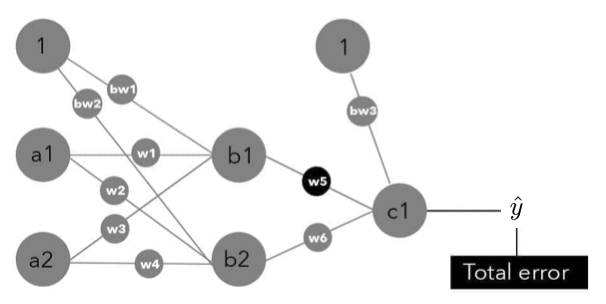
\includegraphics[width=3.5in]{figures/simple_nn_gradient.png}
    \caption{Simple Neural Network \cite{taylor2017neural}} \label{fig:gradient_nn}
\end{figure}

For this example, we will calculate the gradient of the weight $w_5$ and weight $w_1$. To calculate the gradient of weight $w_5$, we need to calculate the rate of change of the total Cross-Entropy with respect to weight $w_5$. Since this simple network only has one output neuron, denoted $c_1$, then the rate of change of total Cross-Entropy is the rate of change of the Cross-Entropy of $\hat{y}$, where $\hat{y}$ is the standardized value of output neuron $c_1$. Thus we have the gradient of weight $w_5$ as:
%
\begin{equation} \label{w5_eq1}
    \frac{\Delta \text{Tot. CE}}{\Delta w_5}= \frac{\Delta \text{CE of }\hat{y}}{\Delta w_5}
\end{equation}
%
However, weight $w_5$ does not affect the Cross-Entropy of $\hat{y}$ directly, but instead affects the net input of output neuron $c_1$, which intern affect the activation signal of $c_1$. Then and only then, output neuron $c_1$ affects the standardized value $\hat{y}$ and its Cross-Entropy. For that reason, to compute the gradient of weight $w_5$, we need to link weight $w_5$ to the Cross-Entropy of $\hat{y}$ by performing chain rule operations on the partial derivative. Apply chain rule to Equation \ref{w5_eq1} for weight $w_5$'s gradient, we have:
%
\begin{equation} \label{w5_eq2}
    \frac{\Delta \text{Tot. CE}}{\Delta w_5}
    = \frac{\Delta \text{CE of }\hat{y}}{\Delta \hat{y}}
    \times \frac{\Delta \hat{y}}{\Delta c_1}
    \times \frac{\Delta c_1}{\Delta c_1 \text{ net\_input}}
    \times \frac{\Delta c_1 \text{ net\_input}}{\Delta w_5}
\end{equation}
%
Similarly to weight $w_5$, the gradient of weight $w_1$ can also be computed using the partial derivative with the chain rule. Weight $w_1$ affects the net input of neuron $b_1$, then its activation signal. Then, neuron $b_1$ impacts the net input of neuron $c_1$ and its activation signal. Neuron $c_1$ then affects $\hat{y}$ and its Cross-Entropy value. Notice that from neuron $c_1$ onward, the change is the same as part of weight $w_5$'s gradient formula; thus, we can expand and adapt Equation \ref{w5_eq2} to compute the gradient of weight $w_1$. The gradient of weight $w_1$ can be evaluated as follow:
%
\[
    \frac{\Delta \text{Tot. CE}}{\Delta w_1} = \frac{\Delta \text{CE of }\hat{y}}{\Delta \hat{y}} \times
    \frac{\Delta \hat{y}}{\Delta c_1} \times \frac{\Delta c_1}{\Delta c_1 \text{ netin}} \times \frac{\Delta c_1 \text{ netin}}{\Delta b_1}
    \times \frac{\Delta b_1}{\Delta b_1 \text{ netin}}
    \times \frac{\Delta b_1 \text{ netin}}{\Delta w_1}
\]
%
where "netin" stand for the net input. These examples showcase the computational process for the gradient of an in-network and an out-network weight, i.e., $w_1$ and $w_5$, respectively. The same computation process for the gradient is applied to all network weights and biases, even with a more complex and higher depth network. Once the gradient is calculated for all the weights and biases, the algorithm knows how much a particular weight or bias changes the network's total error and is thus ready to update each weight and bias accordingly.

\subsection{Backpropagation}
\textbf{Backpropagation} refers to a phase in which the algorithm uses gradients of weight or bias to update their value and bring the network's total error to the global minimum \cite{taylor2017neural}. Since the gradient gives the slope of the loss function with respect to weight or bias, and backpropagation updates their value to approach a local or global minimum, thus gradient descent along with backpropagation process enables the neural network to have a behavior similar to the idea of learning through the process of optimizing network's parameters. The formula to update the value of weight $w_j$ is:
%
\begin{equation} \label{backprop_func}
    \text{new } w_j = \text{old } w_j - \left( \frac{\Delta \text{Tot. CE}}{\Delta w_j} \times \eta \right)
\end{equation}
%
where old $w_j$ is the current value of weight $w_j$, $\frac{\Delta \text{Tot. CE}}{\Delta w_j}$ is the gradient of weight $w_j$, and $\eta$ refers to the algorithm's learning rate.

\textbf{Learning rate}, denoted $\eta$, is a network's hyperparameter, and it determines how fast the network learns. In the updating weight function, equation \ref{backprop_func}, the learning rate directly affects the size of the step when the algorithm moves toward the global minimum for total error. A large learning rate means a bigger step toward minimum, thus resulting in faster learning, while a smaller learning rate value results in slower learning \cite{taylor2017neural}. However, a large learning rate can also affect the network's ability to reach the global minimum, as it can overstep and pass the optimal value. Studies have shown the value of a leaning rate for a multi-layer ANN should be between $10^{-16}$ and 1 with a reasonable default value of 0.01 \cite{bengio2012practical}.

As the backpropagation phase is completed, all weights and biases in the network are updated, and all four phases of the algorithm are repeated on the next batch, where the size of each batch depends on the method of gradient descent. These phases are repeated until the algorithm's total error function reaches a global minimum \cite{taylor2017neural}. At that moment, a test set is passed through the network, and the network's total error is used to evaluate the performance of the network.